%%
%% CubeScope SoftwareX submission draft.
%% Based on the official SoftwareX original software publication template
%% downloaded from the SoftwareX Guide for Authors on 2026-04-24.
%%

\documentclass[preprint,12pt,a4paper]{elsarticle}

\usepackage{amssymb}
\usepackage{graphicx}
\usepackage{hyperref}
\setlength{\parindent}{0pt}
\emergencystretch=2em

\journal{SoftwareX}

\begin{document}
\renewcommand{\labelenumii}{\arabic{enumi}.\arabic{enumii}}

\begin{frontmatter}

\title{CubeScope: a browser-native, local-first viewer kernel for ENVI hyperspectral datasets}

\author{Yongyin Leon Li}
\address{[To be completed with full postal addresses and country names]}

\begin{abstract}
CubeScope is a browser-native viewer kernel for ENVI hyperspectral datasets.
The software targets a gap between heavyweight desktop or server-centered
remote-sensing environments and lightweight web image viewers by providing
local-first, embeddable interaction with multi-band image cubes in modern
browsers. CubeScope combines a Rust/WebAssembly ENVI parser, Web Workers for
background loading and tile-oriented runtime work, and a hardware-accelerated
rendering path that prefers WebGPU while retaining a verified WebGL
compatibility fallback. The current alpha release supports local ENVI loading,
HTTP range-backed remote ENVI access, normalized cube metadata, spectral
probing, affine pixel-to-world coordinate mapping from ENVI spatial metadata,
and explicit runtime packaging for worker and WebAssembly assets. To support
reuse and evaluation, the repository also provides deterministic test fixtures,
public sample validation, benchmark commands, browser smoke tests, packaging
checks, and release-gating reports anchored to a reproducible Node 22
toolchain. Additional local validation on six real ENVI datasets, ranging from
17.6 MB to 381.1 MB, produced successful initial views in all repeated
browser-load trials, with five runs per dataset. CubeScope is intentionally
scoped as an embeddable viewer kernel rather than a full analysis platform,
allowing downstream web applications to integrate hyperspectral browsing
without adopting a heavyweight backend stack.
\end{abstract}

\begin{keyword}
hyperspectral \sep ENVI \sep visualization \sep WebGPU \sep WebAssembly \sep remote-sensing \sep scientific-software
\end{keyword}

\end{frontmatter}

\section*{Required Metadata}

\section*{Current code version}

\begin{table}[!h]
\resizebox{\textwidth}{!}{%
\begin{tabular}{|l|p{6.5cm}|p{6.5cm}|}
\hline
\textbf{Nr.} & \textbf{Code metadata description} & \textbf{Please fill in this column} \\
\hline
C1 & Current code version & 0.1.0-alpha.1 \\
\hline
C2 & Permanent GitHub link to code/repository used for this code version & \url{https://github.com/yongyin-leon/CubeScope/releases/tag/v0.1.0-alpha.1} \\
\hline
C3 & Legal Code License & MIT \\
\hline
C4 & Code versioning system used & git \\
\hline
C5 & Software code languages, tools, and services used & JavaScript, Rust, WebAssembly, Web Workers, WebGPU, WebGL, Vite, Playwright, Vitest \\
\hline
C6 & Compilation requirements, operating environments \& dependencies & Node 22.x, npm 10 or later, Rust toolchain with wasm32-unknown-unknown target, wasm-bindgen-cli 0.2.100; modern browser with WebGL and optional WebGPU \\
\hline
C7 & If available Link to developer documentation/manual & Repository README plus docs/API.md, docs/ARCHITECTURE.md, docs/REPRODUCIBILITY.md \\
\hline
C8 & Support email for questions & [To be completed] \\
\hline
\end{tabular}
}
\caption{Code metadata (mandatory)}
\end{table}

\section{Motivation and significance}

Hyperspectral data are widely used across remote-sensing and imaging
applications, but their high spectral dimensionality still creates practical
inspection and interaction challenges \cite{signoroni2019,ghamisi2017}. In many
applied workflows, access to hyperspectral cubes is mediated by desktop
applications, notebook scripts, or server-oriented geospatial systems. These
approaches remain useful, but they are often too heavy for one increasingly
common task: quickly opening, inspecting, and embedding multi-band image cubes
inside scientific web applications. Many research and engineering teams can
preprocess ENVI data offline, yet still lack a reusable browser-side viewer
that preserves format semantics and supports practical interaction.

CubeScope addresses this gap as a viewer kernel rather than as a complete
analysis platform. The current software artifact focuses on browser-native,
local-first ENVI viewing with a small embeddable API, validated rendering
paths, and reproducibility-oriented release practice. This scope is narrow on
purpose. The present contribution is not a full remote-sensing workbench, but a
reusable foundation for scientific web applications that need hyperspectral
viewing without immediately adopting a heavyweight backend stack.

This positioning also distinguishes CubeScope from adjacent web-facing
hyperspectral systems such as HSIToolbox, which targets the higher-level
problem of server-side hyperspectral classification workflows with dataset
management, labeling, remote training, and multi-user queueing
\cite{dhaene2023}. CubeScope is aimed at a different layer: a browser-native,
local-first viewer kernel that can be embedded into downstream applications,
including future systems that may add classification or analysis services above
it.

\section{Software description}

\subsection{Software architecture}

The public package is \texttt{@cubescope/web}, and the main public class is
\texttt{CubeViewer}. The primary loading contract is \texttt{load(source)}, with
two current source modes: \texttt{envi-local} for paired local files and
\texttt{envi-http} for remote ENVI data served with browser-visible CORS and
HTTP range. The ENVI support is anchored to the format's paired ASCII header
and flat binary image model, including header fields such as interleave,
wavelength, and default-band metadata \cite{nv5header,nv5image}. Within this
scope, the alpha supports pseudo-RGB viewing, band switching, normalized header
access, spectral probing, explicit unloading, and pixel/world coordinate
mapping when ENVI spatial metadata is present.

The initial display band selection is intentionally conservative. CubeScope
uses valid ENVI \texttt{default bands} metadata when available, otherwise it
uses wavelength metadata to choose visible RGB-like bands when the spectrum
covers the visible range, or a spread false-color triplet for non-visible
spectral ranges. If neither metadata source is available, the runtime falls
back to a safe bounded default. This prevents small-band datasets from
requesting out-of-range bands while giving richer datasets a more informative
first view.

CubeScope is organized as a layered browser software stack. The public SDK
exposes a compact class-based interface. Beneath that surface, a viewer runtime
coordinates loading, events, workers, view updates, and renderer interaction.
Below the runtime, data access and format-specific services translate raw
source bytes into normalized cube metadata and read operations. Rendering then
consumes prepared raster and view state rather than direct source-format
details.

\begin{figure}[!ht]
\centering
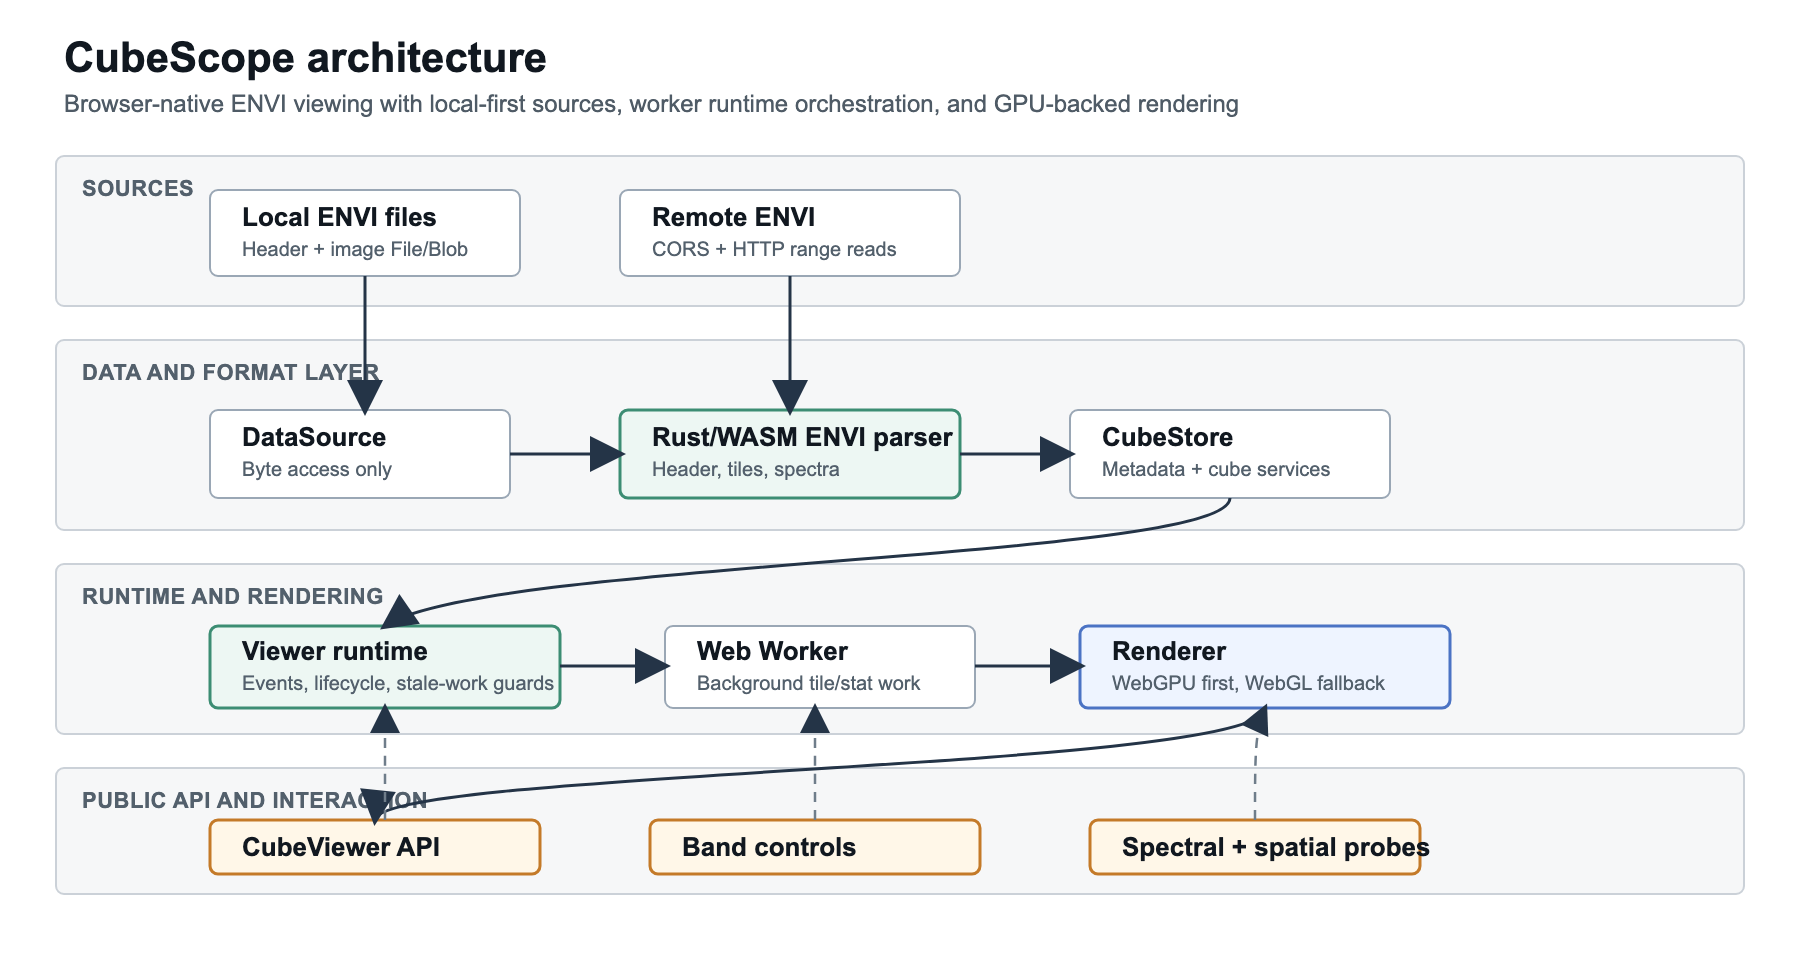
\includegraphics[width=\linewidth]{../figures/softwarex-architecture.png}
\caption{CubeScope architecture. Local and HTTP-range ENVI sources are reduced
to byte access, interpreted through the Rust/WebAssembly ENVI parser, exposed
through normalized cube services, orchestrated by the viewer runtime and worker
layer, and rendered through WebGPU or WebGL behind the public
\texttt{CubeViewer} API.}
\end{figure}

The main architectural seams are \texttt{DataSource}, \texttt{FormatAdapter},
\texttt{CubeStore}, \texttt{Renderer}, and the runtime orchestration shell.
\texttt{DataSource} is responsible for byte access only, currently through
local file/blob reads and an HTTP-range remote path. \texttt{FormatAdapter}
interprets ENVI source bytes, parses metadata, and now provides concrete tile
and spectrum extraction methods backed by shared ENVI cube-read helpers.
\texttt{CubeStore} exposes normalized metadata and cube-oriented services such
as tile reads, spectrum reads, sampled statistics, and pixel/world mapping.
Worker requests rebuild this store and execute through that read model, so the
worker remains a protocol and cancellation boundary rather than the owner of
ENVI byte-layout logic.
\texttt{Renderer} consumes prepared raster layers and view state and is
explicitly separated from source parsing and format semantics.

\subsection{Software functionalities}

The implementation combines Rust/WebAssembly, Web Workers, and browser GPU
rendering in a practical way. ENVI parsing is anchored in a Rust/WebAssembly
component that serves as the authoritative parser layer for the current format
support. Background work is routed through Web Workers using explicit message
envelopes and source-aware request tracking, which helps isolate stale work
when sources change. Rendering is WebGPU-preferred but retains a validated
WebGL compatibility and recovery path. In \texttt{auto} mode, the viewer prefers WebGPU but can
recover through WebGL after a device-loss event, including cases where the
browser requires the render canvas to be recreated before a new graphics
context can be used.

Spatial support follows a conservative but useful boundary. ENVI
\texttt{map info} and \texttt{coordinate system string} fields are normalized
into \texttt{CubeHeader.spatialReference}, and where possible the software
derives an affine transform that powers \texttt{pixelToWorld()} and
\texttt{worldToPixel()} in zero-based image pixel space. Projection descriptors
such as datum, zone, hemisphere, units, and coordinate-system strings are
preserved as metadata, but the current alpha does not infer EPSG identifiers,
apply rotation tokens, or perform full coordinate reference system conversion
or real-time reprojection.

Reproducibility is treated as part of the software contribution. CubeScope uses
Node 22.x as the official release and reproducibility baseline, while newer
Node versions may still be used for local development. In the current validated
local environment, the repository was checked under Node v22.22.2, npm 10.9.7,
and a Rust toolchain with the wasm32-unknown-unknown target plus
wasm-bindgen-cli 0.2.100.

\section{Illustrative examples}

The simplest CubeScope workflow is local ENVI loading. A downstream application
creates a \texttt{CubeViewer}, initializes it, and calls \texttt{load()} with
the header and data files. Once loaded, the viewer exposes normalized metadata,
renders a pseudo-RGB view, allows band switching, and returns a spectral
profile for pixel inspection.

The same viewer contract also supports remote ENVI access through HTTP range.
In that case the source is described by \texttt{headerUrl} and \texttt{dataUrl}
rather than local file handles. This path still depends on browser-visible CORS
and HTTP range, but it allows a web application to interact with ENVI data
without first downloading the full data object eagerly.

When ENVI spatial metadata is present, the application can also retrieve
pixel/world mappings through \texttt{pixelToWorld()} and
\texttt{worldToPixel()}. This supports coordinate-aware inspection while
keeping the render path anchored to source pixel space.

For manuscript preparation, the example application was also exercised with six
local real ENVI datasets, including agricultural, urban, wetland, airborne
near-infrared, and UAV hyperspectral scenes. These cases are used as
illustrative validation examples rather than redistributed test assets. The
resulting screenshots show that the first rendered view is non-blank and
visually interpretable across BIP and BSQ layouts, floating-point and unsigned
integer data, and both metadata-poor and wavelength-described headers.
Candidate provenance sources for these local validation cases include the
Indian Pines/Purdue MultiSpec source \cite{purdueindian}, the EHU/GIC Pavia and
KSC benchmark collection \cite{ehugic}, Resonon Pika IR-L documentation for the
near-infrared sensor family \cite{resononpika}, and the WHU-Hi LongKou
publication \cite{zhong2020}.

\section{Impact}

The current evaluation is a software-release check rather than a full systems
benchmark study. The goal is to show that browser-native hyperspectral
interaction is practical and reproducible. Benchmark reports were generated in
a macOS environment using Node v22.22.2, Chromium 147.0.7727.15, and a
deterministic ENVI fixture with dimensions 48 x 48 x 32.

The benchmark harness records three early metrics: header parse time, time to
initial view, and band-switch time. In the local-file scenario, the measured
values are approximately 6.5 ms, 17.1 ms, and 3.0 ms, respectively. In the
same-origin remote scenario using HTTP range, the values are approximately
5.5 ms, 21.3 ms, and 5.5 ms. These are reported as direct validation outputs,
not as polished comparative benchmarks.

The browser-matrix report adds evidence for renderer behavior. In the current
local Chromium verification, both a forced WebGL scenario and an auto scenario
passed. In the auto scenario, the recorded renderer state shows an observed
transition from WebGPU to WebGL after a device-loss event, with the session
completing in a recovered state. This is not yet a broad browser or hardware
comparison, but it does show that the compatibility path is exercised through
an actual browser workflow.

To complement the deterministic fixture, six real ENVI datasets were loaded
through the example application using Chromium, \texttt{renderer=webgl}, and
\texttt{benchmark=1}. Each case was run five times on the same local machine,
and Table~\ref{tab:real-envi} reports the median and interquartile range of
time to initial view. All cases reached an initial rendered view in all five
runs.

\begin{table}[!ht]
\centering
\resizebox{\textwidth}{!}{%
\begin{tabular}{|l|l|l|l|l|l|l|r|r|}
\hline
Dataset & Dimensions & Interleave & Type & Data size & Spatial & RGB bands & Runs & Initial view ms \\
\hline
Indian Pines & 145 x 145 x 220 & bip & f32 & 17.6 MB & no & 30/20/10 & 5/5 & 45.4 (7.1) \\
\hline
Pavia University & 340 x 610 x 103 & bip & f32 & 81.5 MB & no & 30/20/10 & 5/5 & 130.3 (4.4) \\
\hline
Pavia Centre & 715 x 1096 x 102 & bip & f32 & 304.9 MB & no & 30/20/10 & 5/5 & 399.0 (4.0) \\
\hline
Kennedy Space Center & 614 x 512 x 176 & bip & f32 & 211.1 MB & no & 30/20/10 & 5/5 & 389.7 (7.0) \\
\hline
Pika IR-L Hyalite Creek & 555 x 1500 x 240 & bip & u16 & 381.1 MB & yes & 180/121/61 & 5/5 & 458.5 (5.4) \\
\hline
WHU-Hi LongKou & 400 x 550 x 270 & bsq & f32 & 226.6 MB & no & 113/68/32 & 5/5 & 27.8 (21.0) \\
\hline
\end{tabular}
}
\caption{Local real ENVI validation cases. Initial-view time is reported as
median (IQR) in milliseconds across five browser loads. Local source data were
used only for manuscript-side validation and are not redistributed with the
software package.}
\label{tab:real-envi}
\end{table}

\begin{figure}[!ht]
\centering
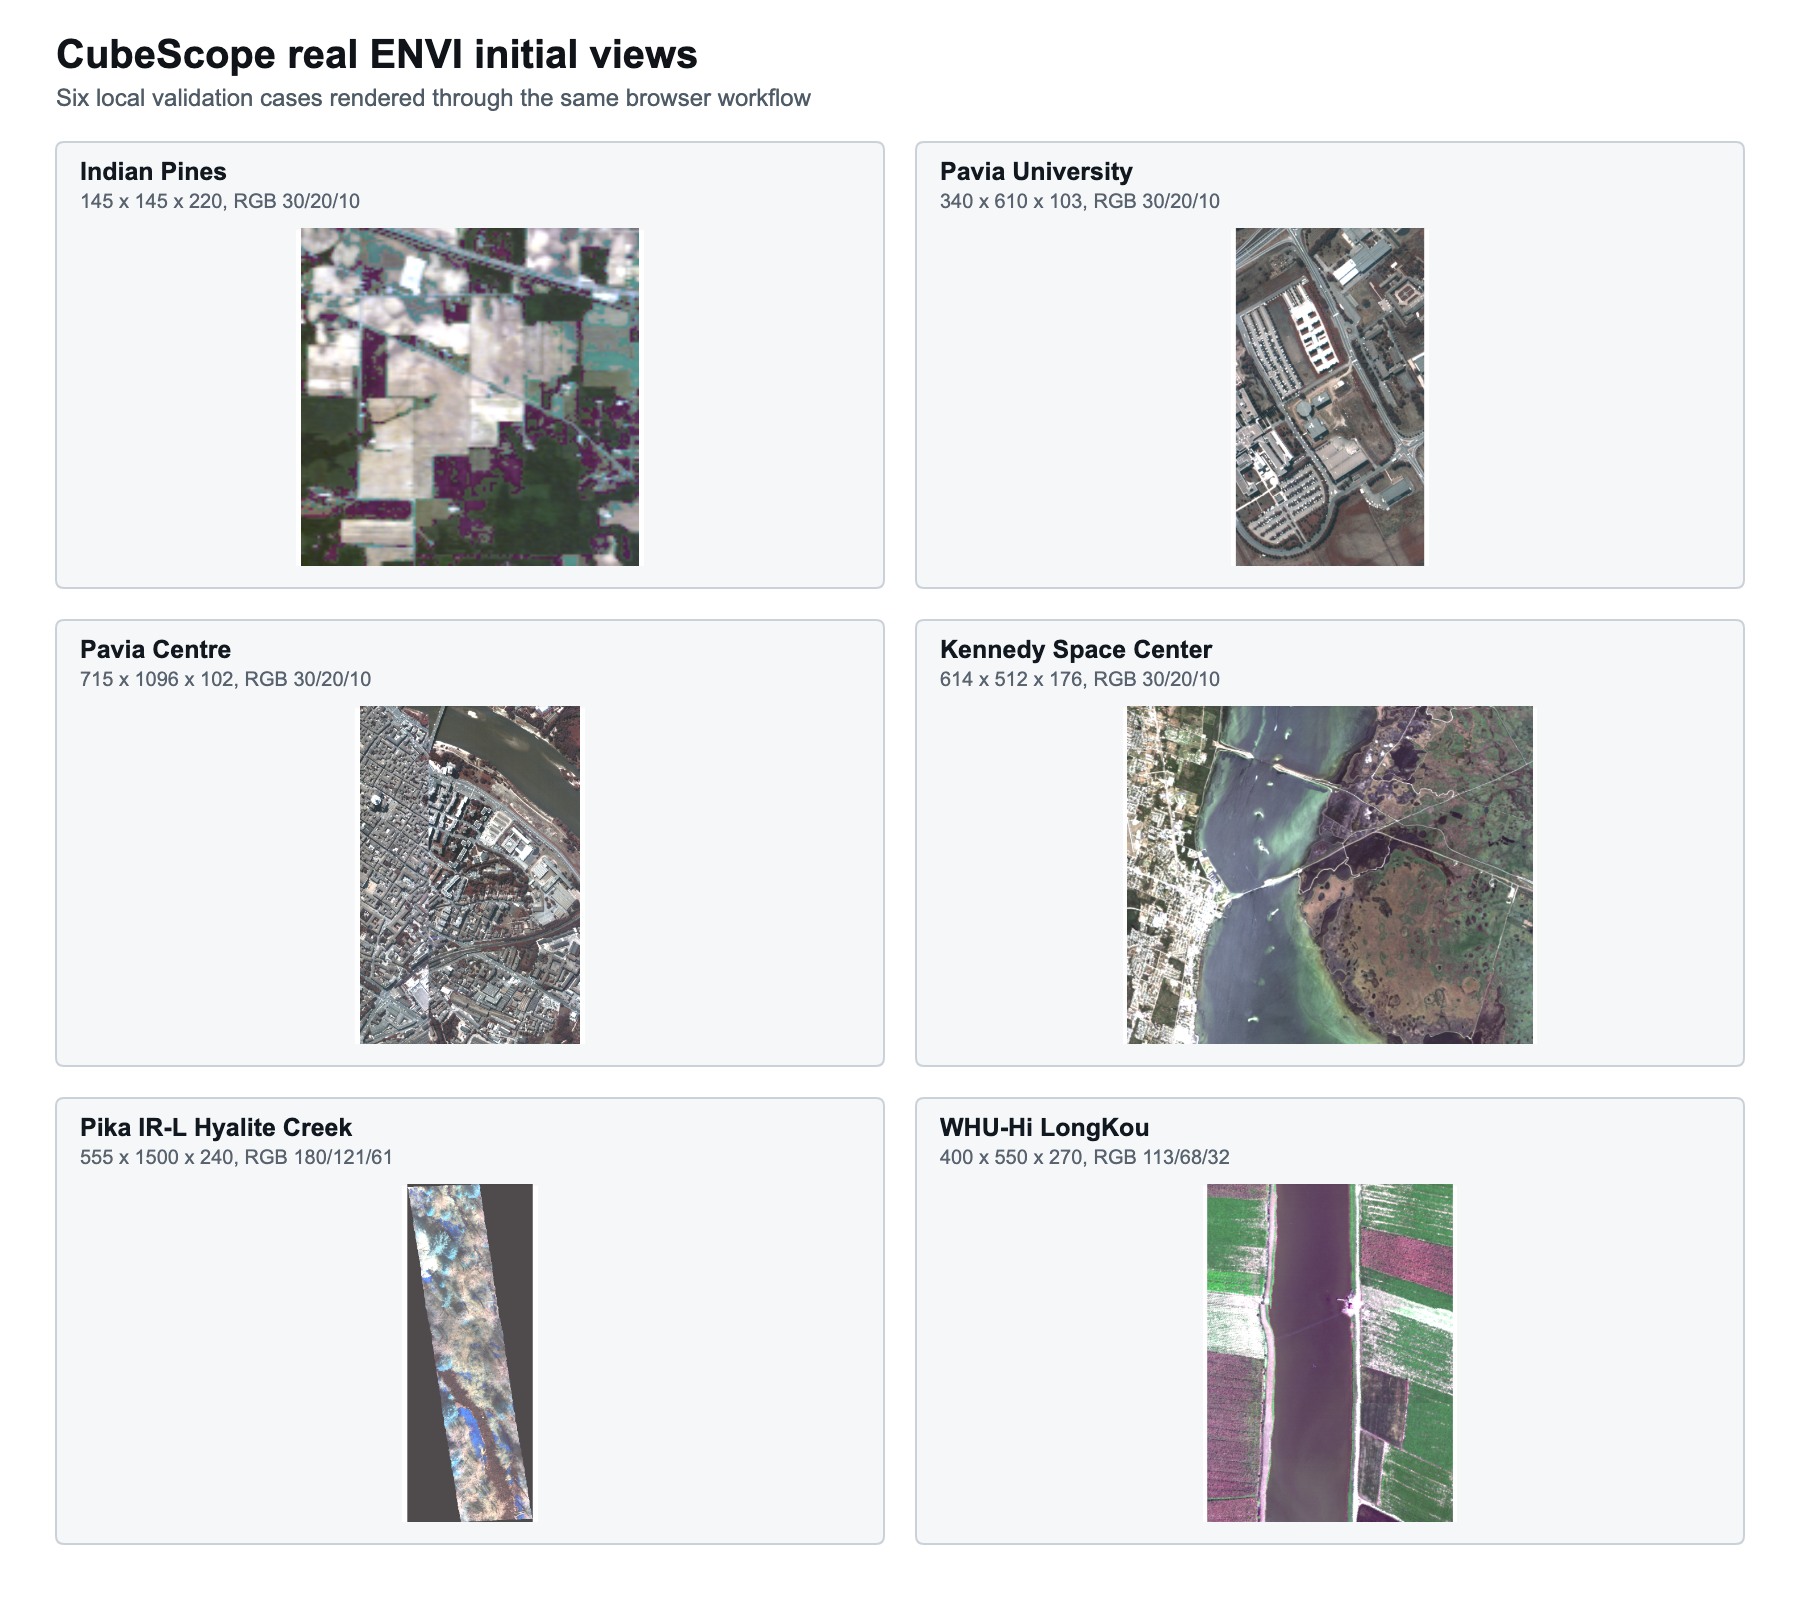
\includegraphics[width=\linewidth]{../figures/softwarex-real-envi-initial-views.png}
\caption{Real ENVI initial views rendered by CubeScope for the six local
validation cases. The panels are generated from browser screenshots of the
example application. Source datasets are used only for manuscript-side
validation and are not redistributed with the software package.}
\end{figure}

These results should be interpreted as practical evidence that the alpha
runtime can open and render varied real ENVI cubes in a browser workflow, not
as a hardware-independent performance claim. Several legacy benchmark datasets
do not provide wavelength or default-band metadata, so their initial colors use
CubeScope's safe pseudo-RGB fallback. The Pika and WHU-Hi cases include
wavelength metadata, and therefore demonstrate the metadata-aware initial band
selection path.

CubeScope lowers the barrier to browser-based hyperspectral viewing. Users and
teams do not need to adopt a heavyweight remote backend or a full desktop
analysis environment simply to inspect ENVI data in a browser. This makes the
software relevant for exploratory work, review interfaces, annotation tools,
quality-control utilities, and educational applications.

The project also has reuse value beyond the repository demo. Because CubeScope
is packaged as a viewer kernel with explicit runtime assets and an embeddable
public API, it can serve as infrastructure for downstream scientific web
applications. The current release also establishes a stable architectural base
for later work on multispectral support, richer spatial overlays, additional
source formats, and lightweight analysis plugins.

The limitations are equally important to state clearly. The software is
currently ENVI-first rather than broadly multi-format. The main artifact is a
browser SDK, so users working only in Python or desktop environments still need
an integration layer. The remote workflow depends on compatible CORS and HTTP
range behavior at the serving endpoint. The benchmark scope is intentionally
narrow and should not be mistaken for a full comparative systems study. The
real-data validation cases were loaded from local files and are not
redistributed with the repository, so their screenshot and timing evidence
should be treated as manuscript-side validation rather than as a complete
public benchmark suite. The current alpha is also not yet a complete scientific
analysis environment.

\section{Conclusions}

CubeScope shows that browser-native hyperspectral viewing can already be
packaged as serious research software without waiting for a full remote-sensing
analysis platform. The current alpha provides a reproducible, embeddable ENVI
viewer kernel built around a Rust/WebAssembly parser, worker-oriented runtime
execution, and hardware-accelerated browser rendering with a validated fallback
path. It pairs that runtime with fixtures, public-sample validation, packaging
checks, benchmark commands, and release-gating reports that improve inspection,
reuse, and citation potential. The additional real ENVI validation cases show
that the same runtime path can produce initial views for selected agricultural,
urban, wetland, airborne, and UAV hyperspectral scenes.

Within its current scope, CubeScope already contributes a meaningful software
base for downstream web applications that need hyperspectral viewing without a
heavy backend stack. Near-term work should widen capability carefully through
multispectral support, richer spatial overlays, additional source adapters, and
later analysis-oriented extensions.

\section*{Data statement}

No new experimental datasets were generated for this software paper. The
repository includes deterministic validation fixtures, benchmark outputs,
browser-matrix reports, sample-validation reports, and packaging-verification
artifacts as part of the software release and reproducibility workflow. Local
real ENVI datasets were used to prepare illustrative screenshots and timing
summaries for the manuscript. The Pavia Centre, Pavia University, and Kennedy
Space Center validation cases were accessed as public benchmark scenes through
the UPV/EHU GIC Hyperspectral Remote Sensing Scenes resource \cite{ehugic}.
Indian Pines is cited through the Purdue MultiSpec/PURR source
\cite{purdueindian}; the local files also match the EHU/GIC index entries, but
Purdue/PURR is treated as the primary provenance source. The Pika IR-L and
WHU-Hi LongKou cases are attributed to the cited source documentation or
publication \cite{resononpika,zhong2020}. These externally obtained source data
files are excluded from Git and are not redistributed with the software
package. If additional submission-system wording is required, this section
should be aligned with the final public repository, release archive, and the
licensing terms of the source datasets.

\section*{Software availability}

Repository: \url{https://github.com/yongyin-leon/CubeScope}\\
Version: 0.1.0-alpha.1\\
License: MIT\\
Primary package: \texttt{@cubescope/web}\\
Permanent software reference: \url{https://doi.org/10.5281/zenodo.20131367}\\
Archived software citation: Li, Y. (2026). CubeScope: browser-native ENVI
hyperspectral viewer kernel. Zenodo.
\url{https://doi.org/10.5281/zenodo.20131367}

\section*{Funding}

[To be completed. If none: This research did not receive any specific grant
from funding agencies in the public, commercial, or not-for-profit sectors.]

\section*{CRediT author statement}

[To be completed using CRediT roles such as Conceptualization, Software,
Validation, Visualization, Writing -- original draft, Writing -- review and
editing, etc.]

\section*{Declaration of competing interest}

The authors declare that they have no known competing financial interests or
personal relationships that could have appeared to influence the work reported
in this paper. [Revise if needed before submission.]

\section*{Declaration of generative AI and AI-assisted technologies in the manuscript preparation process}

[Include this section only if disclosure is required under the final author
decision. Suggested pattern: During the preparation of this work the author(s)
used [NAME OF TOOL / SERVICE] in order to [REASON]. After using this
tool/service, the author(s) reviewed and edited the content as needed and
take(s) full responsibility for the content of the published article.]

\section*{Acknowledgements}

The author acknowledges the UPV/EHU Grupo de Inteligencia Computacional (GIC)
Hyperspectral Remote Sensing Scenes resource, collected by M. Grana, M. A.
Veganzons, and B. Ayerdi, for making benchmark scene information and download
links available to the community. The Pavia Centre and Pavia University scenes
are acknowledged as provided by Prof. Paolo Gamba and the Telecommunications
and Remote Sensing Laboratory, University of Pavia. The Indian Pines data
source is acknowledged through Purdue MultiSpec and the Purdue University
Research Repository. The Kennedy Space Center scene is acknowledged as NASA
AVIRIS data with ground-reference preparation summarized by the EHU/GIC
resource. [Add any funding-specific, institutional, or personal
acknowledgements before final submission.]

\begin{thebibliography}{00}

\bibitem{signoroni2019}
A. Signoroni, M. Savardi, A. Baronio, S. Benini, Deep Learning Meets
Hyperspectral Image Analysis: A Multidisciplinary Review, Journal of Imaging
5(5) (2019) 52. \url{https://doi.org/10.3390/jimaging5050052}

\bibitem{ghamisi2017}
P. Ghamisi, N. Yokoya, J. Li, W. Liao, S. Liu, J. Plaza, B. Rasti, A. Plaza,
Advances in hyperspectral image and signal processing: A comprehensive
overview of the state of the art, IEEE Geoscience and Remote Sensing Magazine
5(4) (2017) 37--78. \url{https://doi.org/10.1109/MGRS.2017.2762087}

\bibitem{dhaene2023}
Z. Dhaene, N. Zizakic, S. Huang, X. Li, A. Pizurica, HSIToolbox: A web-based
application for the classification of hyperspectral images, SoftwareX 22
(2023) 101340. \url{https://doi.org/10.1016/j.softx.2023.101340}

\bibitem{nv5header}
NV5 Geospatial, ENVI Header Files, ENVI Documentation, accessed 2026-04-24.
\url{https://www.nv5geospatialsoftware.com/docs/enviheaderfiles.html}

\bibitem{nv5image}
NV5 Geospatial, ENVI Image Files, ENVI Documentation, accessed 2026-04-24.
\url{https://www.nv5geospatialsoftware.com/docs/ENVIImageFiles.html}

\bibitem{purdueindian}
Purdue University MultiSpec, Hyperspectral Images, Indian Pine Test Site AVIRIS
data, Purdue University Research Repository DOI 10.4231/R7RX991C, accessed
2026-04-24.
\url{https://engineering.purdue.edu/~biehl/MultiSpec/hyperspectral.html}

\bibitem{ehugic}
Grupo de Inteligencia Computacional, University of the Basque Country,
Hyperspectral Remote Sensing Scenes, accessed 2026-04-24.
\url{https://www.ehu.eus/ccwintco/index.php?title=Hyperspectral_Remote_Sensing_Scenes}

\bibitem{resononpika}
Resonon, Pika IR-L (925--1700nm), accessed 2026-04-24.
\url{https://resonon.com/Pika-IR-L}

\bibitem{zhong2020}
Y. Zhong, X. Hu, C. Luo, X. Wang, J. Zhao, L. Zhang, WHU-Hi: UAV-borne
hyperspectral with high spatial resolution (H2) benchmark datasets and
classifier for precise crop identification based on deep convolutional neural
network with CRF, Remote Sensing of Environment 250 (2020) 112012.
\url{https://doi.org/10.1016/j.rse.2020.112012}

\end{thebibliography}

\section*{Current executable software version}

\begin{table}[!h]
\resizebox{\textwidth}{!}{%
\begin{tabular}{|l|p{6.5cm}|p{6.5cm}|}
\hline
\textbf{Nr.} & \textbf{Executable metadata description} & \textbf{Please fill in this column} \\
\hline
S1 & Current software version & 0.1.0-alpha.1 \\
\hline
S2 & Permanent link to executables of this version & \url{https://github.com/yongyin-leon/CubeScope/releases/tag/v0.1.0-alpha.1} and \url{https://doi.org/10.5281/zenodo.20131367} \\
\hline
S3 & Legal Software License & MIT \\
\hline
S4 & Computing platforms/Operating Systems & Browser SDK tested locally on macOS with Chromium; intended for modern browsers with WebGL and optional WebGPU \\
\hline
S5 & Installation requirements \& dependencies & Node 22.x, npm 10 or later for development/build; browser runtime assets bundled with package \\
\hline
S6 & If available, link to user manual & README and docs/API.md \\
\hline
S7 & Support email for questions & [To be completed] \\
\hline
\end{tabular}
}
\caption{Executable software metadata}
\end{table}

\end{document}
